\documentclass[12pt]{article}

\usepackage[margin=1in]{geometry}
\usepackage{amsmath,amsthm,amssymb}
\usepackage{nccmath}
\usepackage{mathtools}
\usepackage{mathrsfs}
\usepackage{enumitem}
\usepackage{physics}
\usepackage{tensor}
\usepackage{subcaption}
\usepackage{pdfpages}

\usepackage{tikz}
\usetikzlibrary{calc,decorations.markings,patterns,math}

\begin{document}

\title{Homework 23}
\author{Sean Ericson \\ Phys 662}
\maketitle

\section*{Problem 1 (Peskin 10.1)}
\[ f_\text{val}(x) = A(1 + ax)(1 - x)^\beta \]
\[ \int_0^1\dd x\; A(1 + ax)(1 - x)^\beta = A\frac{a + \beta + 2}{\beta^2 + 3\beta + 2} = n_q \]
\begin{enumerate}[label=(\alph*)]
    \item The equation above was solved in mathematica with $n_q = 2$ for $u$ and $n_q = 1$ for $d$, with the results in the table below.
    \begin{table}[h]
        \centering
        \begin{tabular}{c c c}
            & $u$ & $d$ \\
            \hline
            $Q = 3.1$ GeV & $A = 9.23$ & $A = 5.56$ \\
            $Q = 100$ GeV & $A = 11.5$ & $A = 6.77$ \\
        \end{tabular}
    \end{table}

    \item Average momentums fractions:
    \begin{table}[h]
        \centering
        \begin{tabular}{c c c}
            & $u$ & $d$ \\
            \hline
            $Q = 3.1$ GeV & $x = 0.351$ & $x = 0.153$ \\
            $Q = 100$ GeV & $x = 0.295$ & $x = 0.187$ \\
        \end{tabular}
    \end{table}

    \item Total momentum fraction:
    \begin{table}[h]
        \centering
        \begin{tabular}{c c}
            & Valence Momentum Fraction \\
            \hline
            $Q = 3.1$ GeV & $x_u + x_d = 0.505$ \\
            $Q = 100$ GeV & $x_u + x_d = 0.482$ \\
        \end{tabular}
    \end{table}
\end{enumerate}

\section*{Problem 2}
\begin{figure*}[h]
    \centering
    \begin{subfigure}[t]{0.5\textwidth}
        \centering
        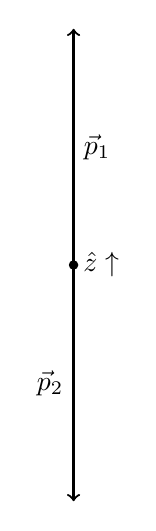
\begin{tikzpicture}
            \tikzmath{\rad = 3;}

            \draw[thick, ->] (0,0)--(0,\rad) node[midway, right]{$\vec{p}_1$};
            \draw[thick, ->] (0,0)--(0,-\rad) node[midway, left]{$\vec{p}_2$};
            \filldraw (0,0) circle[radius=1.5pt] node[right]{$\hat{z}\uparrow$};
        \end{tikzpicture}
        \caption{}
        \label{2jet}
    \end{subfigure}%
    ~ 
    \begin{subfigure}[t]{0.5\textwidth}
        \centering
        \begin{tikzpicture}
            \tikzmath{\rad = 3;}

            \draw[thick, ->] (0,0)--(0,\rad) node[midway, right]{$\vec{p}_1$};
            \draw[thick, ->] (0,0)--({\rad*cos(210)}, {\rad*sin(210)}) node[midway, above]{$\vec{p}_2$};
            \draw[thick, ->] (0,0)--({\rad*cos(-30)}, {\rad*sin(-30)}) node[midway, above]{$\vec{p}_3$};
            \draw[white] (0,0)--(0,-\rad);
            \filldraw (0,0) circle[radius=1.5pt] node[right, yshift=5]{$\hat{z}\uparrow$};
        \end{tikzpicture}
        \caption{}
        \label{3jet}
    \end{subfigure}
    \caption{(a) A 2-jet event. (b) A 3-jet event.}
\end{figure*}

For this problem I will refer to ``directional thrust'', which I'll define as
\[ \tau(\hat{n}) \coloneqq \sum_i \abs{\vec{p}_i \cdot \hat{n}}, \]
such that the actual thrust is given by 
\[ \tau = \frac{\max_{\hat{n}}\tau(\hat{n})}{\sum_i \abs{\vec{p}_i}}. \]

\begin{enumerate}[label=(\alph*)]
    \item
    Choose a coordinate system such that $\hat{n}_0 = \hat{z}$, such as depicted in Figure \ref{2jet}. Denote the common magnitude of the vectors by $p$. By the symmetry of the event, the directional thrust is maximized in the $\pm\hat{z}$ directions (and minimized in directions orthogonal to $\hat{z}$.) Therefore, the thrust is given by
    \[ \tau = \frac{\abs{\vec{p}_1\cdot\hat{n}} + \abs{\vec{p}_2\cdot\hat{n}}}{\abs{\vec{p_1}} + \abs{\vec{p_2}}} = \frac{\abs{p} + \abs{-p}}{2p} = 1  \] 

    \item
    Choose a coordinate system as in part (a), and again denote the magnitude of the vectors by $p$. Again, by the symmetry of the event, the directional thrust is maximized in the $\pm \hat{z}$ directions (or, equivalently, in the directions parallel to $\vec{p}_2$ or $\vec{p}_3$). Noting that 
    \[ \abs{\vec{p}_2\cdot\hat{z}} = \abs{\abs{\vec{p}_2}\cos\frac{2\pi}{3}} = \abs{-\frac{1}{2}\abs{\vec{p}_2}} = \frac{p}{2}, \]
    and similarly for $\vec{p}_3$, we have that the thrust is
    \[ \tau = \frac{p + \frac{p}{2} + \frac{p}{2}}{3p} = \frac{2}{3} \]

    \item
    For a spherically symmetric event, we can evaluate the directional thrust in any direction to get the full thrust. Choosing the $\hat{z}$ direction,
    \[ \tau(\hat{z}) = \int \dd\Omega \abs{\vec{p}\cdot\hat{z}} = 2\pi\int_0^\pi\sin\theta\dd\theta\;\abs{\vec{p}}\abs{\cos\theta} = 2\pi p. \]
    Therefore,
    \[ \tau = \frac{2\pi p}{\int\dd\Omega\abs{\vec{p}}} = \frac{2\pi p}{\int\dd\Omega p} = \frac{2\pi p}{4\pi p} = \frac{1}{2} \]
\end{enumerate}


\section*{Problem 3}
\begin{enumerate}[label=(\alph*)]
    \item 
    \begin{align*}
        \comm{\Sigma_at_R^at_R^a}{t_R^b} &= \Sigma_a\left(t_R^a\comm{t_R^a}{t_R^b} + \comm{t_R^a}{t_R^b}t_R^a\right) \\
        &= \Sigma_{ac}f^{abc}\left(t_R^at_R^c + t_R^ct_R^a\right) \\
        &= 0
    \end{align*}
    The last equality comes from the fact that the structure constants are antisymmetric in the contracted indices ($a$ and $c$), while the object it's contracted with (the anticommutator of $t_R^a$ and $t_R^c$) is symmetric in those indices.
    \item (see attached pdf)
    \item (see attached pdf)
\end{enumerate}
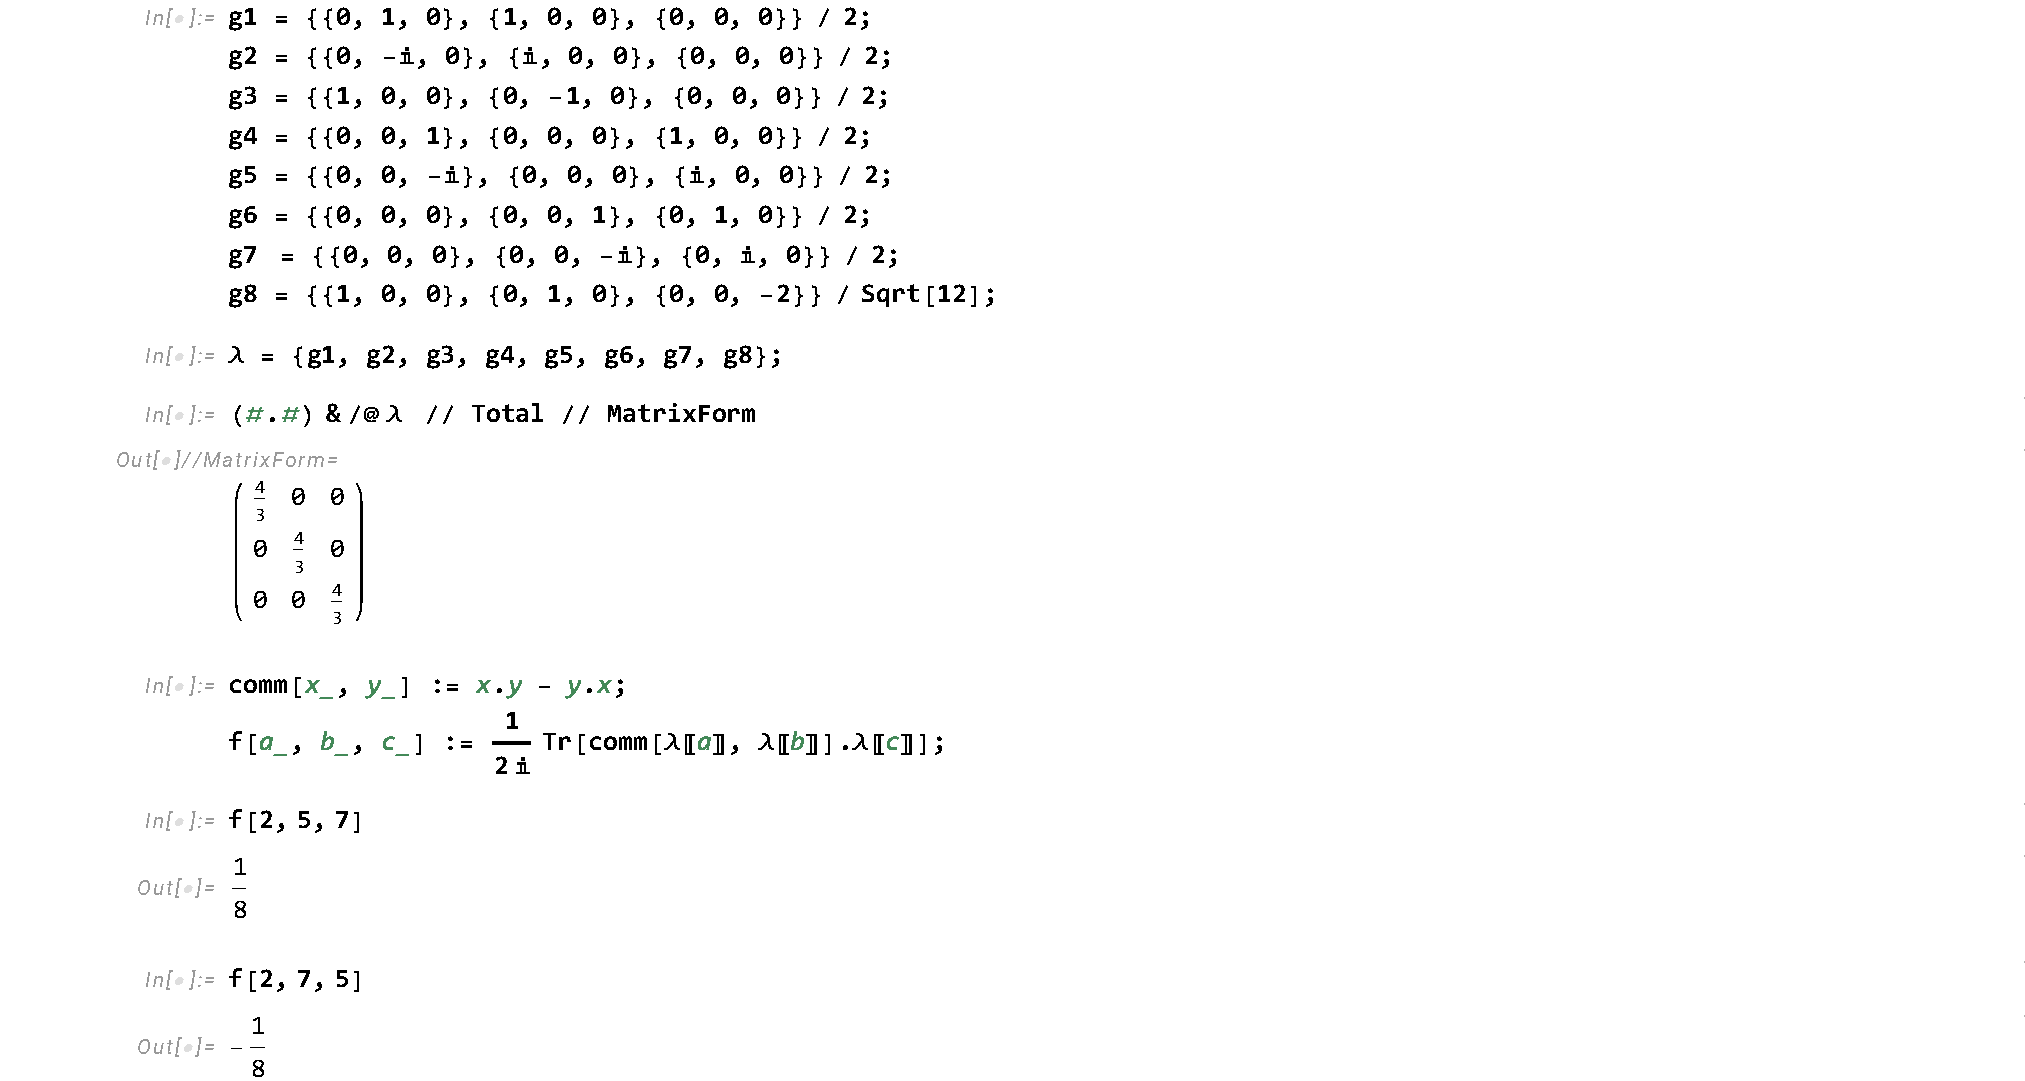
\includepdf[pages=-]{prob3.pdf}

\end{document}